\documentclass[twocolumn]{webofc}
\usepackage[varg]{txfonts}   % Web of Conferences font
\usepackage{booktabs}
\usepackage{array} %% needed for advanced table manipulation
\usepackage{subfigure}
%% Column types from http://tex.stackexchange.com/questions/54069/table-with-text-wrapping
\newcolumntype{L}[1]{>{\raggedright\let\newline\\\arraybackslash\hspace{0pt}}m{#1}}
\newcolumntype{C}[1]{>{\centering\let\newline\\\arraybackslash\hspace{0pt}}m{#1}}
\newcolumntype{R}[1]{>{\raggedleft\let\newline\\\arraybackslash\hspace{0pt}}m{#1}}

\graphicspath{{graphics/}{graphics/arch/}{Graphics/}{./}} % Look in these folders for graphics

\begin{document}
%
\title{PHYS2255 Final Project:\\ Advanced Machine Learning Approaches for Signal-Background Discrimination in Z' Particle Search}
%
% subtitle is optionnal
%
%%%\subtitle{Do you have a subtitle?\\ If so, write it here}

\author{\firstname{Patrick} \lastname{Dobranowski}}

\institute{Vanderbilt University, Nashville, TN}

\abstract{
The goal of this project was to explore various machine learning approaches to the field of particle physics which was discussed at various points throughout the year and presented on many times in lecture by Professor Gurolla. Specifically, Deep Neural Network (DNN) techniques were used to explore beyond the Standard Model (BSM) phenomena with a focus on the detection of the Z' particle, a hypothesized heavy neutral gauge boson. The Z' (U(1)') particle has been proposed as a potential explanation of anomalies found in B-meson decays and presents an interesting challenge due to the similarity of expected standard model processes and those potentially involving the Z' particle. The classification of information from LHC collisions as expected Standard Model (SM) background or signal relating to the Z' particle is what motivates the use of machine learning techniques given the complexity of the data to analyze.
}

%
\maketitle
%
\section*{Introduction.}\label{sec:readme}
This project builds on top of and diverges from an original study performed using XGBoost that studied production of the Z' boson, with family non-universal couplings at the LHC. The referenced study presents a comprehensive feasibility analysis using machine learning techniques of proton-proton collisions considering Z' decays into a pair of third-generation quarks employing these techniques to perform signal-background discrimination to enhance sensitivity to potential signals amidst the background noise of standard model (SM) processes. This project studies the same data with equivalent assumptions aligning with the original goal with an alternative approach to data analysis using Deep Neural Networks (DNNs) as opposed to the Gradient Boosted Decision Trees (XGBoost) of the original work.\cite{Barbosa_2022} This is done to explore the potential application of DNNs in the space of particle physics and high energy physics while taking advantage of the capability of DNNs to model intricate non-linear relationships within large datasets.\\

The data used for these techniques was graciously provided by fellow student Umar Sohail Qureshi.\\

It is important to note, however, that due to time constraints of the project, the models were not able to be trained for extensive periods of time over sufficient epochs. Thus the data presented in this project is not an accurate representation of the potential of these techniques in the specific problem of signal-background classification but rather a representation of an initial exploration in applying DNNs to this complex task.

\section*{Setup.}\label{sec:readme}
All training and all rounds of the various DNN techniques attempted were run on an NVIDIA A100 v4-series GPU on an Azure Virtual Machine providing the computational power necessary for the intensive training cycles.

The data used represents a 47 dimensional data set with the following physical significances:

pT (Transverse Momentum) Columns:

pT b1, pT b2, pT b3, pT b4: These represent the transverse momentum (momentum perpendicular to the beam direction) of the bottom quarks (b-quarks).
pT l: The transverse momentum of a lepton (electron, muon, or tau). This could be a decay product of a top quark.
pT j1, pT j2: The transverse momentum of jets. Jets are streams of particles produced by the hadronization of quarks and gluons.

sdEta (Pseudo-rapidity Difference) Columns:

sdEta b1 b2, sdEta b1 b3, and so on: These are the differences in pseudo-rapidity (a measure related to the angle of the particle relative to the beam direction) between pairs of b-quarks.
sdPhi (Azimuthal Angle Difference) Columns:

sdPhi b1 b2, sdPhi b1 b3, and so on: These represent the differences in the azimuthal angle (angle in the transverse plane) between pairs of particles.
dR (Delta R) Columns:

dR b1 b2, dR b1 b3, and so on: Delta R is a measure of separation between particles in the detector. It's calculated using the differences in pseudo-rapidity and azimuthal angle. Smaller values of dR indicate particles are closer together in the detector.
MET (Missing Transverse Energy):

MET: Represents the missing transverse energy in the event, which is crucial for inferring the presence of non-detected particles like neutrinos.
M (Invariant Mass) Columns:

M b1 b2, M b1 b3, and so on: These are the invariant masses of pairs of particles. The invariant mass is an important quantity in particle physics, as it's conserved in collisions and decays, and can be used to identify the production of certain particles.
MT (Transverse Mass) Columns:

MT l MET, MT b1 l MET, and so on: These represent the transverse mass, calculated using the transverse momentum and missing transverse energy. It's often used in analyses involving neutrinos.

\section*{Methods.}\label{sec:readme}
Three distinct DNN architectures were employed as part of the project: a Multilayer Perceptron (MLP), a Long Short-Term Memory (LSTM) network, and a Convolutional Neural Network (CNN).

The first technique employed, a Multilayer Perceptron, is a type of feedforward neural network designed with 2-3 dense layers consisting of 32-64 neurons employing the Rectified Linear Unit (ReLU) activation function. This simple type of architecture is particularly effective for structured data like ours where features represent distinct physical measurements. To mitigate overfitting, dropout layers were incorporated between the hidden layers which randomly deactivate a portion of the neurons during training to force learning more robust features. The model was also trained using the Adam optimizer and binay cross-entropy loss function which are the most common choices for binary classification tasks as the one presented.

The second technique employed, an LSTM network, is a type of recurrent neural network (RNN) best suited at tackling sequential data. LSTMs are designed to recognize patterns in sequences of data and while the data being analyzed may not be explicitly temporal, comparing other results to those of an LSTM could prove beneficial in the case that sequential relationships in the collected data make a stronger impact than anticipated. For this purpose, to utilize LSTM, the data was reshaped with each feature being treated as a time step adapting the initially 47 dimensional data into an LSTM compatible structure. Return sequences were employed in the initial LSTM layers as expected of an RNN followed by 1-2 dense output layers with a sigmoid activation function being used as opposed to the ReLU of earlier.

The third technique employed, a 1D Convolutional Neural Network, is a technique often used for image data but can also process sequential data in a 1 dimensional manner with greater effectiveness in cases where local data points can more greatly influence the results of a particular classification. The architecture was comprised of convolutional layers that extract these local patterns in the data, pooled to reduce dimensionality, and flattened to enable classification through dense layers. Similar to the MLP of before the CNN was trained using the Adam optimizer with binary cross-entropy loss and dropout for regularization. CNNs have already been used extensively in Particle Physics research and experiments, particularly for images collected by ATLAS experiments but can also be effectively used for non-image data as described.\cite{Ayyar_2020}

\section*{Comparison of Techniques.}\label{sec:readme}
Each of these techniques presents unique benefits that can enhance the performance of the classification model depending on the significance of various parameters in the data. The original methods employing XGBoost for classification suffer from many detriments in the cases of flexibility and feature interaction. While XGBoost is powerful for many classification tasks, it may not capture as complex of relationships as DNN techniques. Additionally, the layered structure of DNNs allows them to automatically learn feature interactions in varying levels of abstraction and offers greater flexibility in terms of architecture design. While XGBoost may provide a range of hyperparameters for tuning, the fundamental architecture of decision trees is fixed and offers less flexibility in enhancements than DNN techniques.

Unfortunately, however, the black box nature of DNNs can give XGBoost an advantage in interpretability through its decision trees but this was not analyzed as part of the results of this project.

\section*{Results.}\label{sec:readme}
Among the more notable of results of this project showed that contrary to the claims of the authors of the initial study, hyperparameter tuning did in fact produce results of significant variance (>1\%). This shows the potential to improve upon previous results using DNNs and several iterations of tuning hyperparameters and architecture structure as opposed to the XGBoost techniques used in the initial study.

Comparing the effectiveness of the various architectures, we see

\begin{figure}[!htb]
    \centering
    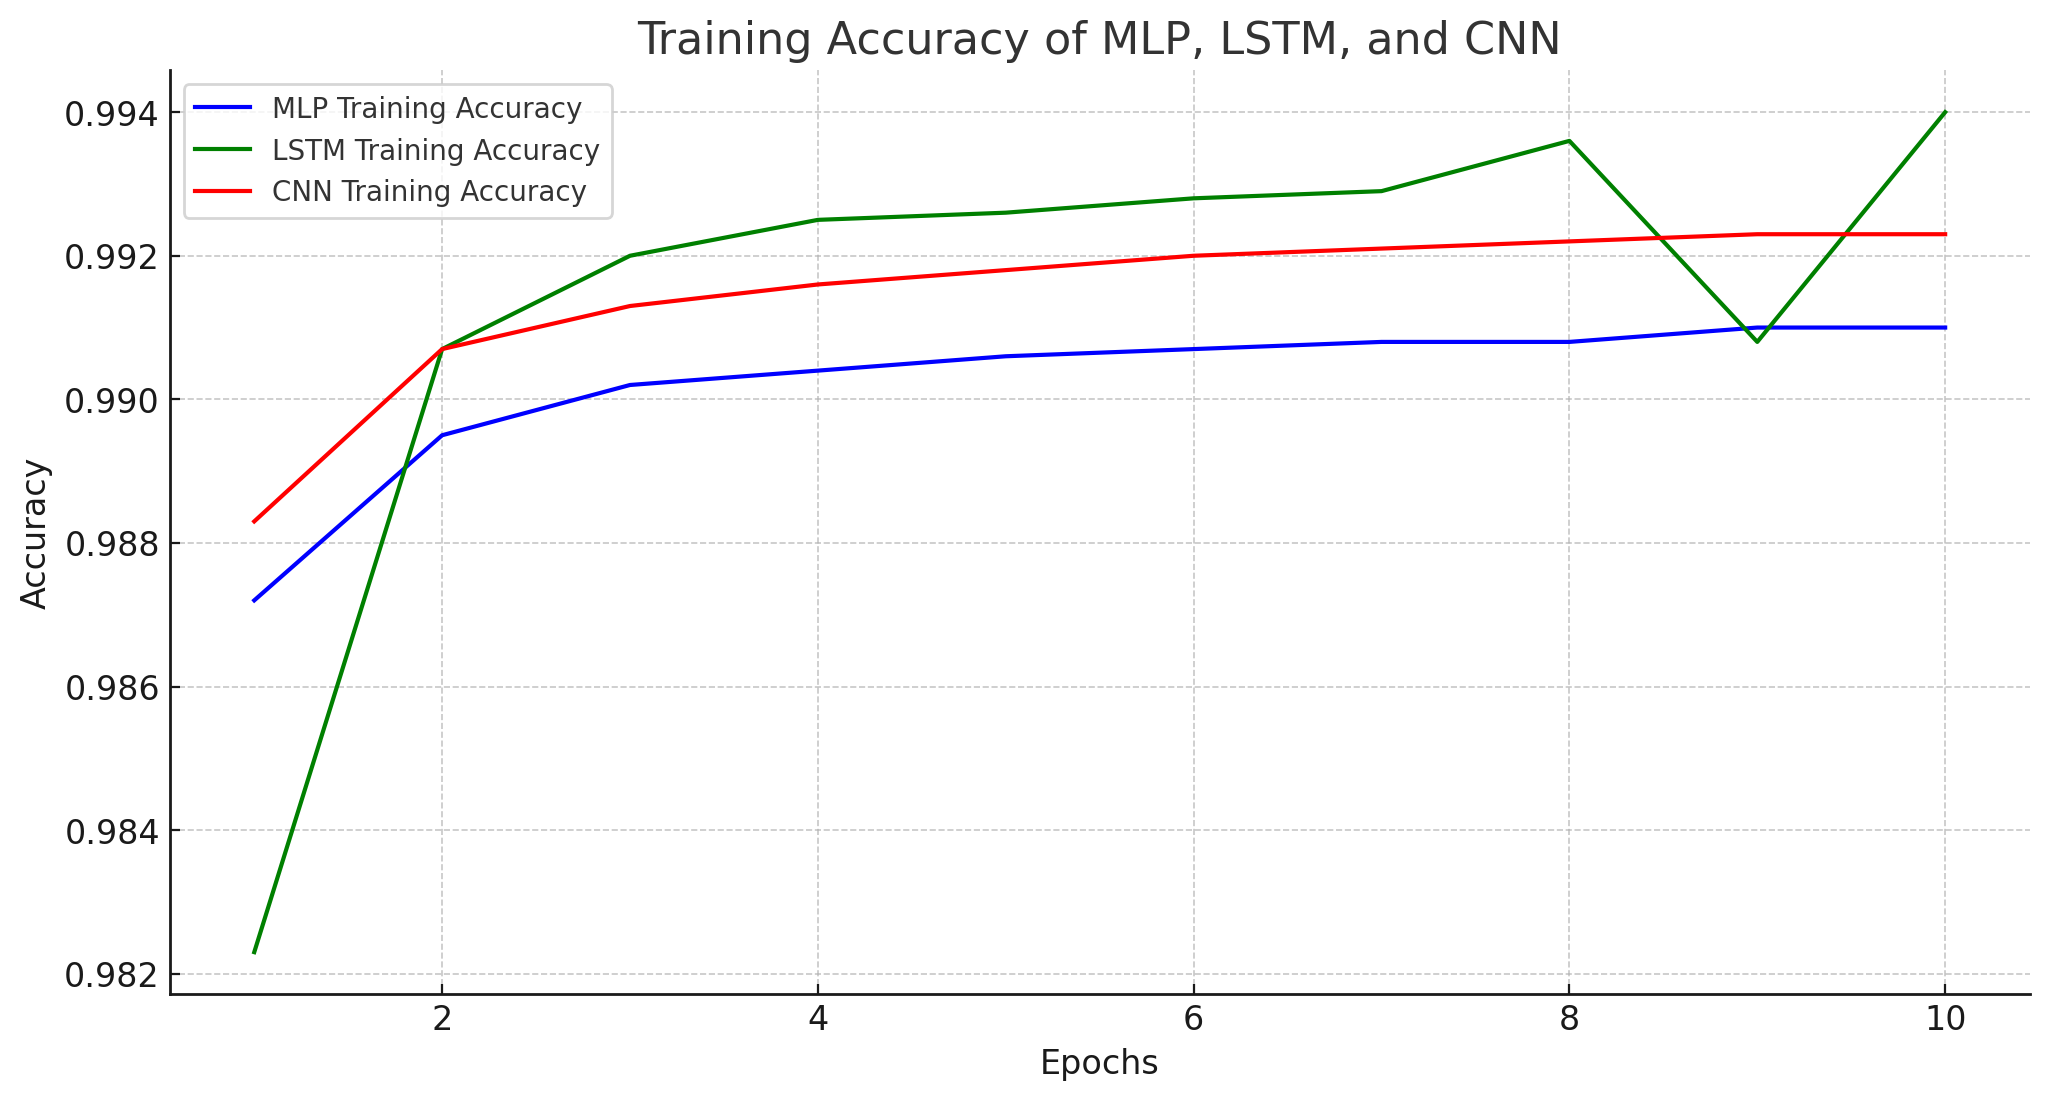
\includegraphics[width=0.5\linewidth]{trainingaccuracy.png}
    \caption{Training Accuracy Across First 10 Epochs}
    \label{fig:enter-label}
\end{figure}

\begin{figure}[!htb]
    \centering
    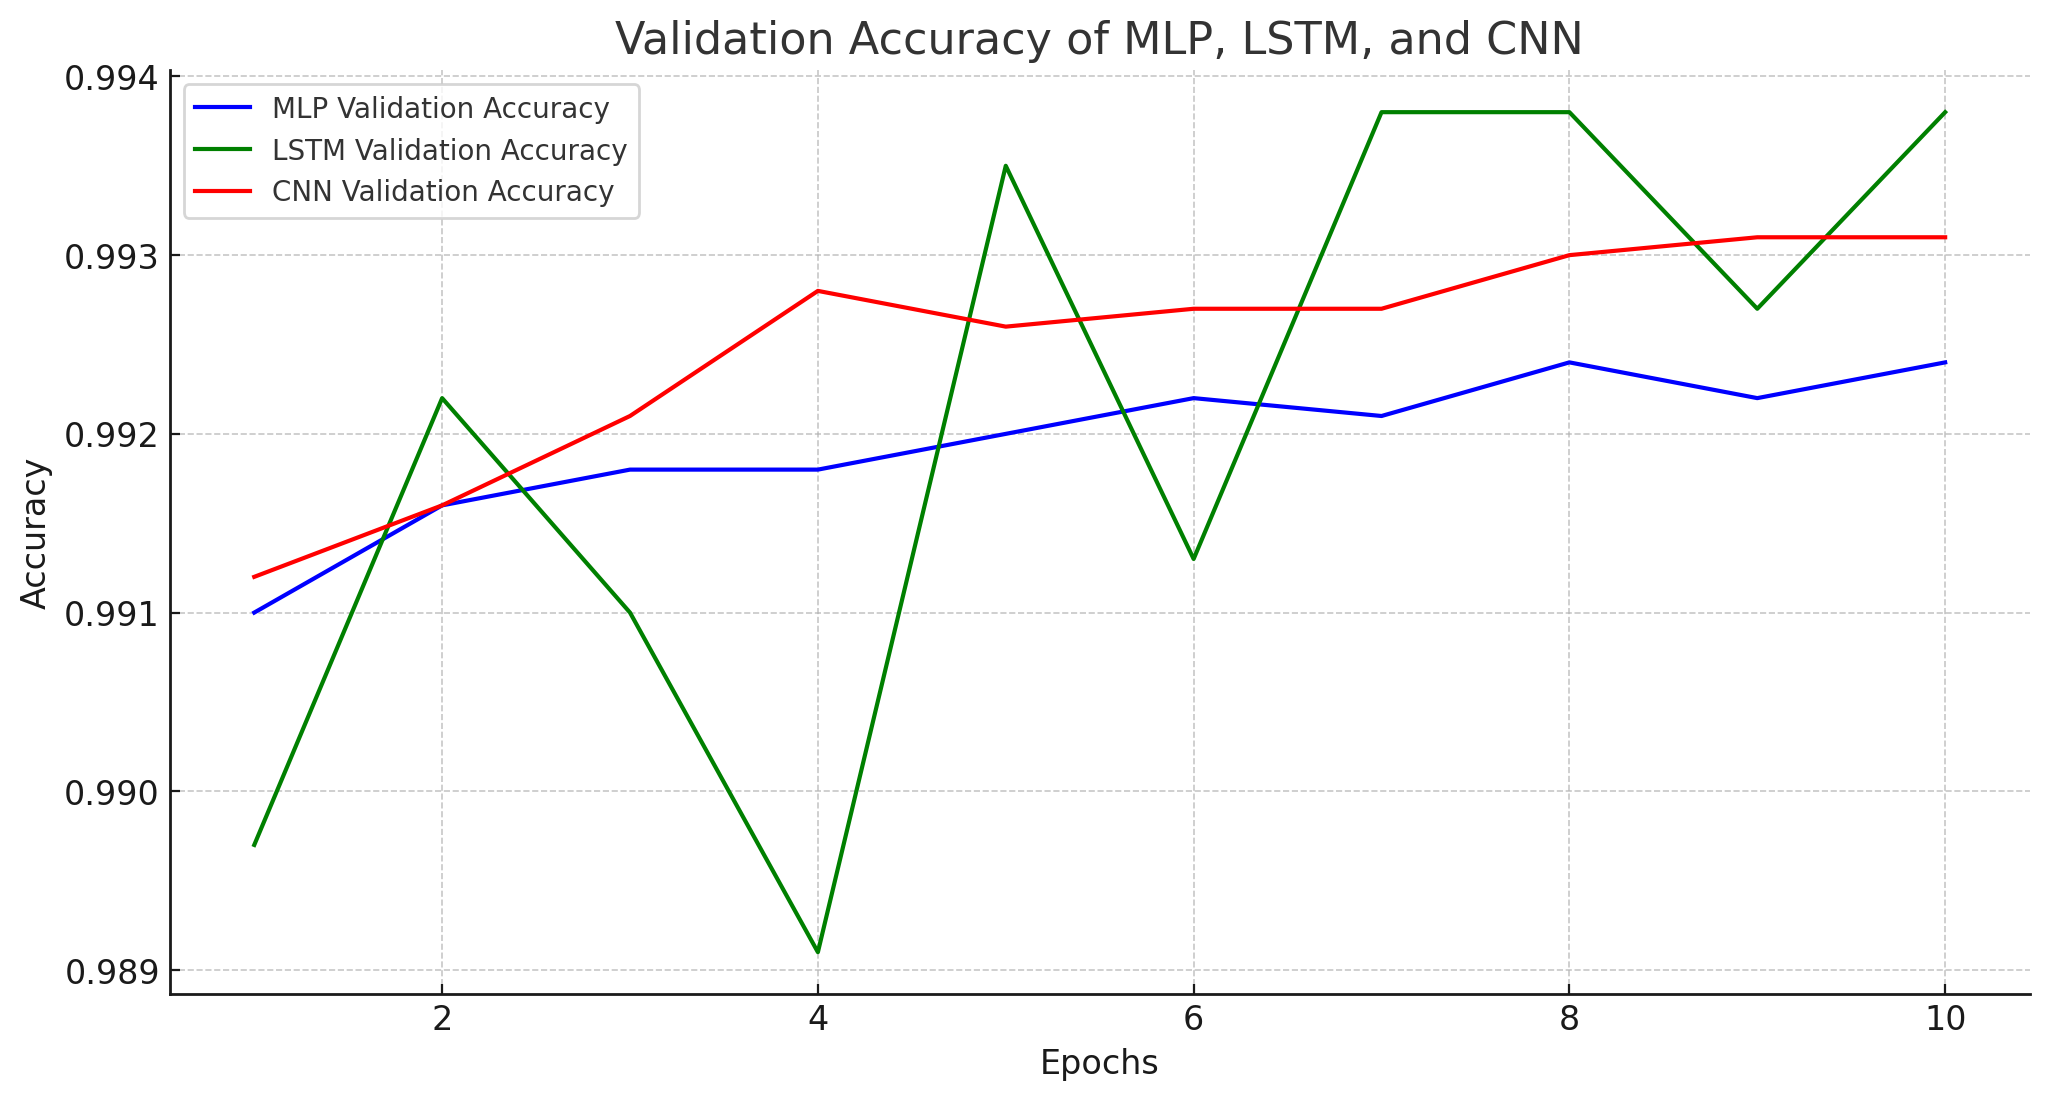
\includegraphics[width=0.5\linewidth]{validationaccuracy-2.png}
    \caption{Validation Accuracy Across First 10 Epochs}
    \label{fig:enter-label}
\end{figure}

The base CNN and LSTM models performed better than the base MLP model prior to any hyperparameter tuning showing that in fact giving increased weight to certain attributes of the data can provide for a better model overall. An accuracy of >99.\% was able to be achieved for each of the models after tuning, with CNN consistently performing better at the base and with LSTM having the best end-performance despite the greatest variance. This quick rise to high performance despite so few epochs showcases the effectiveness of using machine learning technologies for working on complex data and the ability of neural networks to find more differences between signal and background than could be identified by pure physical reasoning. 

Thus, variants of the models presented with further training and tuning of hyperparameters could be used in discriminating Z' particle > quark-antiquark, lepton-antilepton, muon-antimuon pair decays from expected SM processes that produce similar particles as part of larger research in search of the proposed Z' particle.

\section*{Analysis.}\label{sec:readme}
This project gave me the opportunity to engage with the realm of particle physics in a new and interesting way. I was able to go beyond our in-class learning and learn about beyond the Standard Model theories and gain a deeper understanding of what attempts at discovery of new particles look like through a literature review prior to even starting the project (even after the in-class discussions on the discovery of the Higgs boson with Professor Gurolla). I also had the opportunity to combine machine learning, a field that I have engaged with in the past from a computer science perspective, to engage with real-world physics data from the LHC on a portion of a larger research project in the area.

All code written as part of the project can be shared upon request if so desired.

\bibliography{references.bib}


\end{document}
